
%% bare_conf.tex
%% V1.4
%% 2012/12/27
%% by Michael Shell
%% See:
%% http://www.michaelshell.org/
%% for current contact information.
%%
%% This is a skeleton file demonstrating the use of IEEEtran.cls
%% (requires IEEEtran.cls version 1.8 or later) with an IEEE conference paper.
%%
%% Support sites:
%% http://www.michaelshell.org/tex/ieeetran/
%% http://www.ctan.org/tex-archive/macros/latex/contrib/IEEEtran/
%% and
%% http://www.ieee.org/

%%*************************************************************************
%% Legal Notice:
%% This code is offered as-is without any warranty either expressed or
%% implied; without even the implied warranty of MERCHANTABILITY or
%% FITNESS FOR A PARTICULAR PURPOSE! 
%% User assumes all risk.
%% In no event shall IEEE or any contributor to this code be liable for
%% any damages or losses, including, but not limited to, incidental,
%% consequential, or any other damages, resulting from the use or misuse
%% of any information contained here.
%%
%% All comments are the opinions of their respective authors and are not
%% necessarily endorsed by the IEEE.
%%
%% This work is distributed under the LaTeX Project Public License (LPPL)
%% ( http://www.latex-project.org/ ) version 1.3, and may be freely used,
%% distributed and modified. A copy of the LPPL, version 1.3, is included
%% in the base LaTeX documentation of all distributions of LaTeX released
%% 2003/12/01 or later.
%% Retain all contribution notices and credits.
%% ** Modified files should be clearly indicated as such, including  **
%% ** renaming them and changing author support contact information. **
%%
%% File list of work: IEEEtran.cls, IEEEtran_HOWTO.pdf, bare_adv.tex,
%%                    bare_conf.tex, bare_jrnl.tex, bare_jrnl_compsoc.tex,
%%                    bare_jrnl_transmag.tex
%%*************************************************************************

% *** Authors should verify (and, if needed, correct) their LaTeX system  ***
% *** with the testflow diagnostic prior to trusting their LaTeX platform ***
% *** with production work. IEEE's font choices can trigger bugs that do  ***
% *** not appear when using other class files.                            ***
% The testflow support page is at:
% http://www.michaelshell.org/tex/testflow/



% Note that the a4paper option is mainly intended so that authors in
% countries using A4 can easily print to A4 and see how their papers will
% look in print - the typesetting of the document will not typically be
% affected with changes in paper size (but the bottom and side margins will).
% Use the testflow package mentioned above to verify correct handling of
% both paper sizes by the user's LaTeX system.
%
% Also note that the "draftcls" or "draftclsnofoot", not "draft", option
% should be used if it is desired that the figures are to be displayed in
% draft mode.
%
\documentclass[conference]{IEEEtran}
% Add the compsoc option for Computer Society conferences.
%
% If IEEEtran.cls has not been installed into the LaTeX system files,
% manually specify the path to it like:
% \documentclass[conference]{../sty/IEEEtran}





% Some very useful LaTeX packages include:
% (uncomment the ones you want to load)


% *** MISC UTILITY PACKAGES ***
%
%\usepackage{ifpdf}
% Heiko Oberdiek's ifpdf.sty is very useful if you need conditional
% compilation based on whether the output is pdf or dvi.
% usage:
% \ifpdf
%   % pdf code
% \else
%   % dvi code
% \fi
% The latest version of ifpdf.sty can be obtained from:
% http://www.ctan.org/tex-archive/macros/latex/contrib/oberdiek/
% Also, note that IEEEtran.cls V1.7 and later provides a builtin
% \ifCLASSINFOpdf conditional that works the same way.
% When switching from latex to pdflatex and vice-versa, the compiler may
% have to be run twice to clear warning/error messages.






% *** CITATION PACKAGES ***
%
%\usepackage{cite}
% cite.sty was written by Donald Arseneau
% V1.6 and later of IEEEtran pre-defines the format of the cite.sty package
% \cite{} output to follow that of IEEE. Loading the cite package will
% result in citation numbers being automatically sorted and properly
% "compressed/ranged". e.g., [1], [9], [2], [7], [5], [6] without using
% cite.sty will become [1], [2], [5]--[7], [9] using cite.sty. cite.sty's
% \cite will automatically add leading space, if needed. Use cite.sty's
% noadjust option (cite.sty V3.8 and later) if you want to turn this off
% such as if a citation ever needs to be enclosed in parenthesis.
% cite.sty is already installed on most LaTeX systems. Be sure and use
% version 4.0 (2003-05-27) and later if using hyperref.sty. cite.sty does
% not currently provide for hyperlinked citations.
% The latest version can be obtained at:
% http://www.ctan.org/tex-archive/macros/latex/contrib/cite/
% The documentation is contained in the cite.sty file itself.






% *** GRAPHICS RELATED PACKAGES ***
%
\ifCLASSINFOpdf
  % \usepackage[pdftex]{graphicx}
  % declare the path(s) where your graphic files are
  % \graphicspath{{../pdf/}{../jpeg/}}
  % and their extensions so you won't have to specify these with
  % every instance of \includegraphics
  % \DeclareGraphicsExtensions{.pdf,.jpeg,.png}
\else
  % or other class option (dvipsone, dvipdf, if not using dvips). graphicx
  % will default to the driver specified in the system graphics.cfg if no
  % driver is specified.
  % \usepackage[dvips]{graphicx}
  % declare the path(s) where your graphic files are
  % \graphicspath{{../eps/}}
  % and their extensions so you won't have to specify these with
  % every instance of \includegraphics
  % \DeclareGraphicsExtensions{.eps}
\fi
% graphicx was written by David Carlisle and Sebastian Rahtz. It is
% required if you want graphics, photos, etc. graphicx.sty is already
% installed on most LaTeX systems. The latest version and documentation
% can be obtained at: 
% http://www.ctan.org/tex-archive/macros/latex/required/graphics/
% Another good source of documentation is "Using Imported Graphics in
% LaTeX2e" by Keith Reckdahl which can be found at:
% http://www.ctan.org/tex-archive/info/epslatex/
%
% latex, and pdflatex in dvi mode, support graphics in encapsulated
% postscript (.eps) format. pdflatex in pdf mode supports graphics
% in .pdf, .jpeg, .png and .mps (metapost) formats. Users should ensure
% that all non-photo figures use a vector format (.eps, .pdf, .mps) and
% not a bitmapped formats (.jpeg, .png). IEEE frowns on bitmapped formats
% which can result in "jaggedy"/blurry rendering of lines and letters as
% well as large increases in file sizes.
%
% You can find documentation about the pdfTeX application at:
% http://www.tug.org/applications/pdftex





% *** MATH PACKAGES ***
%
%\usepackage[cmex10]{amsmath}
% A popular package from the American Mathematical Society that provides
% many useful and powerful commands for dealing with mathematics. If using
% it, be sure to load this package with the cmex10 option to ensure that
% only type 1 fonts will utilized at all point sizes. Without this option,
% it is possible that some math symbols, particularly those within
% footnotes, will be rendered in bitmap form which will result in a
% document that can not be IEEE Xplore compliant!
%
% Also, note that the amsmath package sets \interdisplaylinepenalty to 10000
% thus preventing page breaks from occurring within multiline equations. Use:
%\interdisplaylinepenalty=2500
% after loading amsmath to restore such page breaks as IEEEtran.cls normally
% does. amsmath.sty is already installed on most LaTeX systems. The latest
% version and documentation can be obtained at:
% http://www.ctan.org/tex-archive/macros/latex/required/amslatex/math/





% *** SPECIALIZED LIST PACKAGES ***
%
%\usepackage{algorithmic}
% algorithmic.sty was written by Peter Williams and Rogerio Brito.
% This package provides an algorithmic environment fo describing algorithms.
% You can use the algorithmic environment in-text or within a figure
% environment to provide for a floating algorithm. Do NOT use the algorithm
% floating environment provided by algorithm.sty (by the same authors) or
% algorithm2e.sty (by Christophe Fiorio) as IEEE does not use dedicated
% algorithm float types and packages that provide these will not provide
% correct IEEE style captions. The latest version and documentation of
% algorithmic.sty can be obtained at:
% http://www.ctan.org/tex-archive/macros/latex/contrib/algorithms/
% There is also a support site at:
% http://algorithms.berlios.de/index.html
% Also of interest may be the (relatively newer and more customizable)
% algorithmicx.sty package by Szasz Janos:
% http://www.ctan.org/tex-archive/macros/latex/contrib/algorithmicx/




% *** ALIGNMENT PACKAGES ***
%
%\usepackage{array}
% Frank Mittelbach's and David Carlisle's array.sty patches and improves
% the standard LaTeX2e array and tabular environments to provide better
% appearance and additional user controls. As the default LaTeX2e table
% generation code is lacking to the point of almost being broken with
% respect to the quality of the end results, all users are strongly
% advised to use an enhanced (at the very least that provided by array.sty)
% set of table tools. array.sty is already installed on most systems. The
% latest version and documentation can be obtained at:
% http://www.ctan.org/tex-archive/macros/latex/required/tools/


% IEEEtran contains the IEEEeqnarray family of commands that can be used to
% generate multiline equations as well as matrices, tables, etc., of high
% quality.




% *** SUBFIGURE PACKAGES ***
%\ifCLASSOPTIONcompsoc
%  \usepackage[caption=false,font=normalsize,labelfont=sf,textfont=sf]{subfig}
%\else
%  \usepackage[caption=false,font=footnotesize]{subfig}
%\fi
% subfig.sty, written by Steven Douglas Cochran, is the modern replacement
% for subfigure.sty, the latter of which is no longer maintained and is
% incompatible with some LaTeX packages including fixltx2e. However,
% subfig.sty requires and automatically loads Axel Sommerfeldt's caption.sty
% which will override IEEEtran.cls' handling of captions and this will result
% in non-IEEE style figure/table captions. To prevent this problem, be sure
% and invoke subfig.sty's "caption=false" package option (available since
% subfig.sty version 1.3, 2005/06/28) as this is will preserve IEEEtran.cls
% handling of captions.
% Note that the Computer Society format requires a larger sans serif font
% than the serif footnote size font used in traditional IEEE formatting
% and thus the need to invoke different subfig.sty package options depending
% on whether compsoc mode has been enabled.
%
% The latest version and documentation of subfig.sty can be obtained at:
% http://www.ctan.org/tex-archive/macros/latex/contrib/subfig/




% *** FLOAT PACKAGES ***
%
%\usepackage{fixltx2e}
% fixltx2e, the successor to the earlier fix2col.sty, was written by
% Frank Mittelbach and David Carlisle. This package corrects a few problems
% in the LaTeX2e kernel, the most notable of which is that in current
% LaTeX2e releases, the ordering of single and double column floats is not
% guaranteed to be preserved. Thus, an unpatched LaTeX2e can allow a
% single column figure to be placed prior to an earlier double column
% figure. The latest version and documentation can be found at:
% http://www.ctan.org/tex-archive/macros/latex/base/


%\usepackage{stfloats}
% stfloats.sty was written by Sigitas Tolusis. This package gives LaTeX2e
% the ability to do double column floats at the bottom of the page as well
% as the top. (e.g., "\begin{figure*}[!b]" is not normally possible in
% LaTeX2e). It also provides a command:
%\fnbelowfloat
% to enable the placement of footnotes below bottom floats (the standard
% LaTeX2e kernel puts them above bottom floats). This is an invasive package
% which rewrites many portions of the LaTeX2e float routines. It may not work
% with other packages that modify the LaTeX2e float routines. The latest
% version and documentation can be obtained at:
% http://www.ctan.org/tex-archive/macros/latex/contrib/sttools/
% Do not use the stfloats baselinefloat ability as IEEE does not allow
% \baselineskip to stretch. Authors submitting work to the IEEE should note
% that IEEE rarely uses double column equations and that authors should try
% to avoid such use. Do not be tempted to use the cuted.sty or midfloat.sty
% packages (also by Sigitas Tolusis) as IEEE does not format its papers in
% such ways.
% Do not attempt to use stfloats with fixltx2e as they are incompatible.
% Instead, use Morten Hogholm'a dblfloatfix which combines the features
% of both fixltx2e and stfloats:
%
% \usepackage{dblfloatfix}
% The latest version can be found at:
% http://www.ctan.org/tex-archive/macros/latex/contrib/dblfloatfix/




% *** PDF, URL AND HYPERLINK PACKAGES ***
%
%\usepackage{url}
% url.sty was written by Donald Arseneau. It provides better support for
% handling and breaking URLs. url.sty is already installed on most LaTeX
% systems. The latest version and documentation can be obtained at:
% http://www.ctan.org/tex-archive/macros/latex/contrib/url/
% Basically, \url{my_url_here}.

%*** para suportar acentuação ***
\usepackage[utf8]{inputenc}

%*** para suportar tabelas com colunas mergeadas ***
\usepackage{multirow}

%*** Para inclusão de imagens e permitir rotacionar texto ***
\usepackage{graphicx}			% Inclusão de gráficos
\graphicspath{ {./} }			% localizando as imagens

%*** Para ajustar a largura das colunas e para multilinhas nas células ***
\usepackage{array}
\newcolumntype{L}{>{\centering\arraybackslash}m{0,75cm}}
\newcolumntype{M}{>{\RaggedLeft\arraybackslash}m{3cm}}

% *** Do not adjust lengths that control margins, column widths, etc. ***
% *** Do not use packages that alter fonts (such as pslatex).         ***
% There should be no need to do such things with IEEEtran.cls V1.6 and later.
% (Unless specifically asked to do so by the journal or conference you plan
% to submit to, of course. )

\usepackage{xcolor}
\newcommand{\marcos}[1]{{\color{blue}{MARCOS: #1}}}
\newcommand{\fancyname}{Dizang}
\newcommand{\fancynameX}{\fancyname}


% correct bad hyphenation here
\hyphenation{op-tical net-works semi-conduc-tor}


\begin{document}
%
% paper title
% can use linebreaks \\ within to get better formatting as desired
% Do not put math or special symbols in the title.
%\title{Coletando dados de memória de máquina em nuvem para análise forense de ataques de injeção de código}
\title{\fancynameX: Uma solução para coleta de evidências forenses de ataques de injeção na nuvem}


% author names and affiliations
% use a multiple column layout for up to three different
% affiliations
\author{\IEEEauthorblockN{Hamilton Fonte II, Marcos A. Simplicio Jr.}
\IEEEauthorblockA{
Escola Politécnica, Universidade de São Paulo (USP)
São Paulo, SP, Brasil\\
Email: hamiltonii@gmail.com, mjunior@larc.usp.br}
%\and
%\IEEEauthorblockN{Marcos A. Simplicio Jr.}
%\IEEEauthorblockA{
%Escola Politécnica -- Universidade de São Paulo (USP)
%São Paulo, SP, Brasil\\
%Email: mjunior@larc.usp.br}
}

% conference papers do not typically use \thanks and this command
% is locked out in conference mode. If really needed, such as for
% the acknowledgment of grants, issue a \IEEEoverridecommandlockouts
% after \documentclass

% for over three affiliations, or if they all won't fit within the width
% of the page, use this alternative format:
% 
%\author{\IEEEauthorblockN{Michael Shell\IEEEauthorrefmark{1},
%Homer Simpson\IEEEauthorrefmark{2},
%James Kirk\IEEEauthorrefmark{3}, 
%Montgomery Scott\IEEEauthorrefmark{3} and
%Eldon Tyrell\IEEEauthorrefmark{4}}
%\IEEEauthorblockA{\IEEEauthorrefmark{1}School of Electrical and Computer Engineering\\
%Georgia Institute of Technology,
%Atlanta, Georgia 30332--0250\\ Email: see http://www.michaelshell.org/contact.html}
%\IEEEauthorblockA{\IEEEauthorrefmark{2}Twentieth Century Fox, Springfield, USA\\
%Email: homer@thesimpsons.com}
%\IEEEauthorblockA{\IEEEauthorrefmark{3}Starfleet Academy, San Francisco, California 96678-2391\\
%Telephone: (800) 555--1212, Fax: (888) 555--1212}
%\IEEEauthorblockA{\IEEEauthorrefmark{4}Tyrell Inc., 123 Replicant Street, Los Angeles, California 90210--4321}}




% use for special paper notices
%\IEEEspecialpapernotice{(Invited Paper)}




% make the title area
\maketitle

% As a general rule, do not put math, special symbols or citations
% in the abstract
\begin{abstract}
A adoção de arquiteturas em nuvem aumenta a cada dia, e com ela também o número de casos em que esse tipo de tecnologia é usada para fins ilícitos. 
%
Infelizmente, devido à natureza volátil da nuvem, a tarefa de coletar evidências para análise forense nesse ambiente tem esbarrado em desafios práticos e legais.
%
Este trabalho analisa propostas na literatura voltadas a resolver os principais desafios existentes na coleta evidências na nuvem, discutindo suas limitações, e então propõe uma solução que cobre coleta, transporte e armazenamento da evidência visando suplantá-las. 
%
A solução aqui proposta provê uma forma de correlacionar evidências e sua origem virtual, permitindo transportar e armazenar tais dados sem afetar sua credibilidade tendo como focos (1) a reprodutibilidade do processo de coleta e (2) a garantia de custódia da evidência.

\end{abstract}

% no keywords




% For peer review papers, you can put extra information on the cover
% page as needed:
% \ifCLASSOPTIONpeerreview
% \begin{center} \bfseries EDICS Category: 3-BBND \end{center}
% \fi
%
% For peerreview papers, this IEEEtran command inserts a page break and
% creates the second title. It will be ignored for other modes.
\IEEEpeerreviewmaketitle

\section{Introdução}

%==== CONTEXTO GERAL: Nuvem e volatilidade de VMs ====
%
Técnicas de virtualização, replicação de serviços e compartilhamento de recursos entre múltiplos usuários (multi-inquilinato) proveem a nuvens computacionais uma elevada escalabilidade \cite{Morsy_Cloud_Security:2010}.
%
Ao mesmo tempo, tais mecanismos também criam uma elevada volatilidade das máquinas virtuais que executam aplicações em nuvem.
%
Afinal, uma aplicação hospedada na nuvem, quando submetida a um pico de uso, pode criar clones das máquinas virtuais que a hospedam e balancear a carga entre elas, de modo a atender à demanda sem prejuízos na qualidade do serviço oferecido. 
%
Após esse pico, e com o objetivo de não incorrer em custos desnecessários, as máquinas que foram clonadas são normalmente desativadas, seus recursos liberados e o sistema retorna à capacidade anterior. 


%==== CONTEXTO ESPECÍFICO + PROBLEMA GERAL: Forense na nuvem vs. volatilidade + multitenancy + multidomains ====
%
Embora interessante do ponto de vista de eficiência e custos, do ponto de vista forense a volatilidade da nuvem traz problemas em caso de ataques.
%
Por exemplo, caso uma das instâncias de máquina virtual criadas temporariamente seja alvo de ameaças que atuam diretamente na sua memória, sem deixar rastros em discos como arquivos de log, as evidências desse evento podem ser completamente perdidas.
%
Essa dificuldade é ainda agravada por aspectos como multi-inquilinato e multi-jurisdição típicas de soluções em nuvem \cite{Bash_Adv_in_Forensics:2015}.
%
Especificamente, o aspecto multi-inquilino dificulta a obtenção do hardware que executa as aplicações de interesse, pois, como ele é compartilhado por vários usuários, removê-los para análise poderia levar a uma violação de privacidade dos usuários não relacionados à investigação. 
%
Já a característica distribuída da nuvem pode levar à alocação de informações relevante à investigação em vários países, dificultando a obtenção das mesmas em especial quando não existem acordos de cooperação entre as instituições e/ou países envolvidos \cite{Dykstra_Acquiring_for_IAAS:2012}.
%
Combinadas, tais características da nuvem dificultam a coleta de evidências com a credibilidade necessária para que elas possam ser usadas em processos legais,  o que exige o respeito à privacidade, à jurisdição e à cadeia de custódia, bem como a reprodutibilidade do processo de coleta \cite{Rahman_Live_Forensics_Techniques:2015}.



%==== O QUE EXISTE E PORQUE NÃO É SUFICIENTE: ??? ====
%
Embora existam soluções na literatura que abordam a coleta de informações de nuvem com o propósito de análise forense, a grande maioria aborda a coleta, o transporte e o armazenamento o faz de forma isolada.
%
Por exemplo, trabalhos como \cite{Dykstra_FROST:2013} e \cite{Reichert_Auto_acquisition:2015} tratam de fatores como multi-inquilinato e multi-jurisdição, discutindo formas de coleta e preservação da evidência fora da núvem.
%
Já estudos como \cite{George_DF2CE:2012} focam na forense ao vivo para a coleta de evidência das máquinas virtuais, enquanto trabalhos como \cite{Sang_Log_approach:2013} aborda a questão de processos de garantia de cadeia de custódia em ambientes de nuvem para transporte da evidência.
%
%abordam os problemas descritos anteriormente \marcos{QUAIS, CARA PÁLIDA? VOCÊ LISTOU 4 TIPOS DE ATAQUE E DEIXOU UM PROBLEMA GERAL: COMO O LEITOR VAI SABER QUAIS EXATAMENTE SÃO ABORDADOS? Seja mais preciso: clareza acima de tudo!!!} de forma isolada.
%
%Alguns propõem soluções para o os fatores multi-inquilino e multi-jurisdição, outros abordam apenas a coleta de evidência de máquinas virtuais e por fim temos as que descrevem apenas os processos de garantia de cadeia de custodia. \marcos{Er... você não me deu sequer um exemplo, então eu sou obrigado a acreditar em você sem que você apresente argumentos... lembre-se que revisores são seres amargos e cruéis, que não acreditam em nada, então melhor não arriscar e dar exemplos claros.}
%
Por outro lado, não foram identificados na literatura propostas de solução que (1) descrevam como o dado é coletado e armazenado observando a cadeia de custódia, e (2) permitam garantir que, mesmo que uma máquina virtual seja desalocada, haja condições de se reproduzir o processo de coleta de evidências.



%==== O QUE FAZEMOS: Ataques de injeção ====
%
O presente trabalho visa suplantar tais limitações por meio de uma proposta que tem como focos (1) a reprodutibilidade do processo de coleta e (2) a garantia de custódia da evidência.
%
Em suma, a abordagem aqui descrita provê uma forma de correlacionar evidências e sua origem virtual, permitindo transportar e armazenar tais dados de modo a preservar sua credibilidade.
%
Esta proposta supõe que o sistema sendo monitorado é executado dentro de um contêiner em nuvem. O foco da solução em contêiner se justifica pelo crescimento da adoção de conteinerização nos últimos anos e a previsão de que este será o mais usado modelo de implementação \cite{Piraghaj_Container_Cloud_Computing:2016}.
%g
A solução tem como alvo específico ataques de injeção de código \cite{Case_Memory_Forensics:2014}, pois estes, quando usados contra uma arquitetura em nuvem, não deixam rastros quando máquinas virtuais são desativadas e seus recursos liberados \cite{Vomel_Memory_Acquisition:2013}, \cite{Case_Memory_Forensics:2014}.
%
Em particular, têm especial interesse quatro tipos específicos dessa família de ameaças \cite{Case_Memory_Forensics:2014}:


\begin{itemize}
 \item \textbf{Injeção remota de bibliotecas}: Um processo malicioso força o processo alvo a carregar uma biblioteca em seu espaço de memória.
 %
 Como resultado, o código da biblioteca carregada executa com os mesmos privilégios do executável em que ela foi injetada. 
 %
 Esta estratégia, comumente usada para instalar malwares, pode fazer com que uma biblioteca maliciosa armazenada no sistema seja distribuída por vários processos de uma mesma máquina, dificultando sua remoção \cite{Miller_Remote_Library_Injection:2004}.
 %
 \item \textbf{Inline Hooking}: Um processo malicioso escreve código como uma sequência de bytes diretamente no espaço de memória de um processo alvo e força este último a executá-lo. 
 %
 O código pode ser, por exemplo, um script de shell.
 %
 \item \textbf{Injeção reflexiva de biblioteca}: Um processo malicioso acessa diretamente a memória de um processo alvo, inserindo nela o código de uma biblioteca na forma de uma sequência de bytes, e então força o processo a executar essa biblioteca. 
 %
 Nesta forma de ataque, a biblioteca maliciosa não existe fisicamente; isso torna esta estratégia de injeção de código potencialmente mais atrativa, pois o carregamento da biblioteca não é registrado no sistema operacional e, portanto, o ataque torna-se mais difícil de ser detectado \cite{Fewer_Reflective_Library_Inject:2008}.
 %
 \item \textbf{Injeção de processo vazio}: Um processo malicioso dispara uma instância de um processo legítimo no estado ``suspenso''; a área do executável é então liberada e realocada com código malicioso.
\end{itemize}


O restante deste documento está organizado da seguinte forma.
%
A Seção \ref{sec:cloud} discute brevemente soluções em nuvem e suas características.
%
A Seção \ref{sec:related} analisa os trabalhos relacionados na área de forense de memória.
%
A Seção \ref{sec:proposal} detalha a solução proposta e avalia como ela trata os desafios alvo deste projeto.
%
Finalmente, a Seção \ref{sec:conclusion} apresenta algumas considerações finais e discute ideias para trabalhos futuros.


\section{Adoção de arquiteturas em nuvem}
\label{sec:cloud}



Nuvem computacional é um modelo de infra estrutura onde recursos compartilhados configuráveis acessíveis via rede são provisionados e descartados com esforço mínimo de gerenciamento ou recurso de um provedor de serviço. \cite{NIST2011}
%A infra-estrutura é composta de máquinas físicas contendo cada uma um número variável de máquinas virtuais que implementam este serviço \cite{Sousa_Computacao_Nuvem:2009}. 
%
Há três modelos principais de comercialização de uso da nuvem \cite{NIST2011}: plataforma como serviço (PaaS) onde se provê infra estrutura para que o cliente instale seu software, software como serviço(SaaS) onde se provê o software que será usado pelo cliente e, o tipo mais pertinente para este trabalho, Infraestrutura como serviço (IaaS) ondê se provê recursos computacionais fundamentais.


Contêiners Linux (LXC), uma tecnologia para auxiliar no gerenciamento de containeres para isolamento de recursos introduzida em 2008, proveram uma série de ferramentas para tirar vantagens das funcionalidades de cgroups e namespacing do kernel do Linux. 
%
A adoção de contêiners para a implantação de software tem crescido muito para nas aplicações baseadas em nuvem. Segundo o ``Container Market Adoption Survey 2016'' realizado pelas empresas DevOps.com (https://devops.com/) e ClusterHQ (https://clusterhq.com) com 235 empresas que tem desenvolvimento de software como sua atividade fim ou como suporte a atividade fim, 76\% dos respondentes utilizam contêiners para melhorar a eficiência do processo de desenvolvimento e em suas arquiteturas de micro serviços em nuvem.

\section{Trabalhos relacionados}
\label{sec:related}

A literatura voltada a analise forense na nuvem foi analisada a luz dos seguintes conceitos. 

\subsection{Acessar e coletar as informações de memória das máquinas virtuais em nuvem}

Referente a coleta de informações, os autores \cite{Reichert_Auto_acquisition:2015}, \cite{Poisel_VMI:2013}, \cite{Dykstra_FROST:2013}, \cite{George_DF2CE:2012} e \cite{Sang_Log_approach:2013} focam em coleta "após o fato" pois ela acontece apenas após a intrusão ser detectada. 
%
Os processos de coleta descritos nos trabalhos são iniciados de forma manual ou automáticamente via integração com um mecanismo de detecção de intrusão. 
%
No caso específico de memória volátil, tal forma de coleta não consegue descrever como era a memória antes da intrusão pois o processo só é acionado depois da detecção do ataque. 
%
A capacidade de saber como era a memória antes do fato é descrita por \cite{Case_Memory_Forensics:2014} como necessária para viabilizar a abordagem de coletar o suficiente para realizar a investigação pois permite comparar dois instantâneos de memória e minimizar o volume coletado antes do fato. 
%
A única proposta encontrada que leva tal necessidade em consideração é \cite{Dezfouli_Backup_approach:2012} mas propõe que o dado seja armazenado no próprio dispositivo porém essa abordagem não é aplicável ao cenário em nuvem pois leva a perda de informações importantes caso a máquina virtual seja despejada e seus recursos liberados.

Ainda na coleta de informações, os autores \cite{Reichert_Auto_acquisition:2015} e \cite{George_DF2CE:2012} sugerem a abordagem de forense ao vivo onde os dados são constantemente coletados sem distinção do antes ou depois do fato. 
%
Os autores \cite{Poisel_VMI:2013}, \cite{Dykstra_FROST:2013} e \cite{Sang_Log_approach:2013} adotam a estratégia de isolar e parar a máquina virtual para em seguida realizar o processo de coleta. 
%
Nas duas estratégias citadas anteriormente, o problema do grande volume de informações coletadas não é abordado pelo autores nem o cenário onde é necessário coletar evidências de uma máquina virtual que já foi despejada do pool e os recursos liberados. 
%
Atender este último cenário é importante pois com as soluções em nuvem que escalam automaticamente, as evidências de uma máquina vítima de um ataque que foi despejada de um pool com a diminuição da demanda serão para sempre perdidas. 

\subsection{Capacidade de reproduzir o processo e obter os mesmos resultados}

A reprodutibilidade do processo de coleta é uma dos requisitos para garantir a cadeia de custódia da evidência e sua aceitação em um processo legal. Cadeia de custódia esta relacionado a credibilidade e ter dois analistas reproduzindo o processo de coleta de memória chegando ao mesmo conjunto de evidências tem um peso muito forte em termos de credibilidade. 
%
Neste tópico, nenhuma das propostas encontradas até o momento consegue reproduzir os mesmos resultados ao repetir o processo no cenário em que uma máquina virtual é despejada da nuvem e seus recursos liberados pois todas elas dependem da existência da máquina virtual para a repetição da coleta. 

\subsection{Não violar privacidade ou jurisdição das partes não envolvidas na investigação}

No caso das soluções em nuvem, não é possível remover o hardware para análise pois ele contem informações de vários usuários, alguns dos quais não estão envolvidos na investigação em curso, fazê-lo levaria a violações de privacidade, o que diminui a credibilidade da evidência. 
%
A maioria dos autores resolve este problema adequadamente e podemos listar duas estratégias usadas. 
%
Os autores \cite{Reichert_Auto_acquisition:2015}, \cite{George_DF2CE:2012}, \cite{Poisel_VMI:2013} e \cite{Dykstra_FROST:2013} usam estratégias de coletar dados pertinentes a investigação e armazená-los fora da nuvem enquanto que \cite{Sang_Log_approach:2013} e um caso específico de \cite{George_DF2CE:2012} dependem da cooperação do provedor de serviços de nuvem para conseguir as informações necessárias à investigação. 
%
Depender do provedor de serviços de nuvem é considerada uma estratégia fraca pela comunidade forense pois o foco do provedor de nuvem é garantir a continuidade do serviço e não a coleta de evidências.

\subsection{Garantir a cadeia de custódia da evidência}

Na garantia da cadeia de custódia apenas \cite{Sang_Log_approach:2013} aborda a questão, mas toma cuidados somente para garantir que a evidência não foi destruída ou alterada através do cálculo de hashing da mesma mas não explica como impede o acesso não autorizado. 
%
As propostas dos outros autores estão focadas apenas no aspecto técnico da coleta, nenhum deles menciona garantia de custódia, apenas que as evidências são coletadas de forma "forensicamente aceitável".

A Tabela 1 mostra um comparativo das soluções estudadas.

\begin{table}[h]
\centering
\caption{Comparativo de soluções de coleta de informações de memória de máquinas em nuvem para análise forense \marcos{LEGENDAS DEVEM SER DESCRITIVAS O SUFICIENTE PARA QUE SEJAM ENTENDIDAS SEM QUE SEQUER EU TENHA LIDO O SEU TEXTO...} }
\begin{tabular}{p{3.0cm}|L|L|L|L}
\cline{2-5}
\textbf{}			& \rotatebox{90}{\textbf{Coleta  é contínua?}}      & \rotatebox{90}{\textbf{Reproduz o processo sem a VM?}} & \rotatebox{90}{\textbf{Garante cadeia de custódia?}}      & \rotatebox{90}{\textbf{Preserva jurisdição e privacidade?}}          \\ \hline
Dizang				& 
\includegraphics[scale=0.015]{check.png}	    & 
\includegraphics[scale=0.015]{check.png}               & 
\includegraphics[scale=0.015]{check.png}                  & 
\includegraphics[scale=0.015]{check.png}                             \\ \hline
DF2CE-George			& 
\includegraphics[scale=0.007]{x.png}		    & 
\includegraphics[scale=0.007]{x.png}                   & 
\includegraphics[scale=0.007]{x.png}                      & 
\includegraphics[scale=0.015]{check.png}                             \\ \hline
VMI-Poisel			& 
\includegraphics[scale=0.007]{x.png}              & 
\includegraphics[scale=0.007]{x.png}                   & 
\includegraphics[scale=0.007]{x.png}                      & 
\includegraphics[scale=0.015]{check.png}                             \\ \hline
FROST-Dykstra			& 
\includegraphics[scale=0.007]{x.png}              & 
\includegraphics[scale=0.007]{x.png}                   & 
\includegraphics[scale=0.007]{x.png}                      & 
\includegraphics[scale=0.015]{check.png}                             \\ \hline
Desafios da Forense-Do		& 
\includegraphics[scale=0.007]{x.png}              & 
\includegraphics[scale=0.007]{x.png}                   & 
\includegraphics[scale=0.007]{x.png}                      & 
\includegraphics[scale=0.015]{check.png}                             \\ \hline
Auto Aquisition-Reichert	& 
\includegraphics[scale=0.007]{x.png}              & 
\includegraphics[scale=0.007]{x.png}                   & 
\includegraphics[scale=0.015]{check.png}                  & 
\includegraphics[scale=0.015]{check.png}                             \\ \hline
Log Approach-Sang		& 
\includegraphics[scale=0.015]{check.png}          & 
\includegraphics[scale=0.007]{x.png}	             & 
\includegraphics[scale=0.015]{check.png}                  & 
\includegraphics[scale=0.015]{check.png}                             \\ \hline
Semantic Gap-Dolan		& 
\includegraphics[scale=0.007]{x.png}              & 
\includegraphics[scale=0.007]{x.png}                   & 
\includegraphics[scale=0.007]{x.png}                      & 
\includegraphics[scale=0.015]{check.png}                             \\ \hline
Comp. Analisys-Aljaedi		& 
\includegraphics[scale=0.007]{x.png}              & 
\includegraphics[scale=0.007]{x.png}                   & 
\includegraphics[scale=0.007]{x.png}                      & 
\includegraphics[scale=0.015]{check.png}                             \\ \hline
Bkp. Approach-Dezfouli		& 
\includegraphics[scale=0.015]{check.png}          & 
\includegraphics[scale=0.007]{x.png}                   & 
\includegraphics[scale=0.007]{x.png}                      & 
\includegraphics[scale=0.015]{check.png}                             \\ \hline
FAAS-VanBaar			& 
\includegraphics[scale=0.015]{check.png}          & 
\includegraphics[scale=0.007]{x.png}                   & 
\includegraphics[scale=0.015]{check.png}                  & 
\includegraphics[scale=0.015]{check.png}                             \\
\end{tabular}
\end{table}

\section{Solução proposta: Dizang}
\label{sec:proposal}

O presente proposta tem como objetivo principal coletar memória de uma máquina virtual de modo a conseguir: 
(1) identificar os quatro tipos de ataque listados anteriormente; 
(2) identificar sua fonte, mesmo se a máquina virtual não existir mais; 
(3) descrever o sistema antes e depois do incidente;
%
Além disso, deve-se armazenar a memória coletada de modo a garantir sua integridade e confidencialidade, sem violar a jurisdição cabível ou a privacidade de outros usuários no mesmo servidor físico.

\subsection{Descrição}

Nas soluções com infra-estrutura física a máquina é persistente. A associação de uma informação da memória, a imagem de um disco ou pacotes trafegando na rede à sua origem é duradoura.
%
Com as soluções de infra virtual, em especial as auto-escaláveis, a máquina deixou de ser persistente e tornou-se volátil. 
%
Para resolver o problema da identificação da fonte é necessário encontrar outro elemento persistente para identificar a fonte da evidência coletada. Para isto usou-se contêineres. 
%
Embora o contêiner seja uma peça de software e por consequência também é volátil, a imagem compilada e sua execução na forma de contêiner estão atrelados a um hash que os identificam unicamente. 
%
A pilha de um contêiner pode ser visto na Figura 1.\\

\begin{figure}[h]
\caption{Pilha monstrando funcionamento de contêiner}
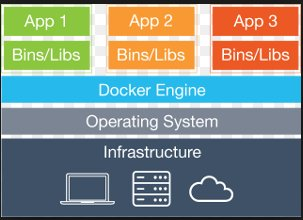
\includegraphics[scale=0.5]{docker.jpg}
\centering
\label{fig:pilha}
\end{figure}

A solução proposta por este trabalho para resolver o problema de associação da evidência a sua origem de modo que o processo seja reprodutível, pausa a execução do contêiner e coleta um instantâneo da memória dos processos sob sua execução. 
%
Esta coleta é executada em intervalos de tempo conhecidos de modo a se um histórico da memória dos processos. Em um sistema derivado do linux (Ubuntu 14.04) isso foi atingido via cópia do diretório ``\\proc'' relacionado aos processos sob o ``cgroup'' associado ao contêiner e salvo em disco. 
%
Para relacionar o instantâneo a sua origem, assinou-se o arquivo em que foram salvos o instantâneo da memória com o hash da imagem como mostrado na Figura 2.\\

\begin{figure}[h]
\caption{Evidência salva - hash do contêiner e imagem}
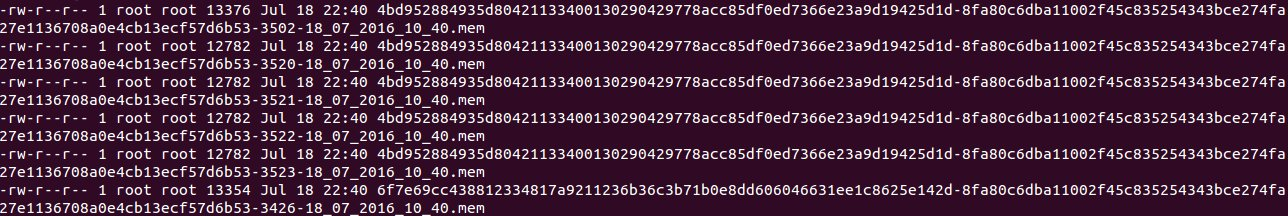
\includegraphics[scale=0.2]{snapshot.jpg}
\centering
\label{fig:instantaneo}
\end{figure}

As técnicas forenses praticadas hoje estão voltadas para a obtenção da informação em sua totalidade, seja via cópia bit a bit, seja por remoção do hardware \cite{Simou_Cloud_Chlng:2014} \cite{Bem_Past_Present_Future:2008}. 
%
Tais práticas tem levado ao crescente volume de dados que os investigadores tem que analisar. Há uma vertente na comunidade chamada ``sniper forensics'' onde se coleta e armazena o suficiente para a investigação. 
%
A solução proposta por este trabalho acompanha esta tendência. 
%
A questão foi definir a quantidade de dados ``suficiente'' para uma investigação. 
%
De acordo com \cite{Case_Memory_Forensics:2014}, detectar intrusões na memória de processos depende de termos uma descrição da memória antes e depois da intrusão. 
%
Com base nisso determinou-se que ``suficiente'' seria a quantidade necessária para descrever o sistema antes e depois do ataque. 
%
A idéia é implementar um log rotativo de instantâneos de memória cobrindo uma quantidade de tempo configurável. Integrar a solução com algum sistema de detecção de ameaça de modo que, ao detectar um ataque, o log passa de rotativo a completo permitindo que se conheça o sistema antes e depois do ataque e sua evolução como mostrado na Figura 3. \\

\begin{figure}[h]
\caption{Janela deslizante de coleta de evidência}
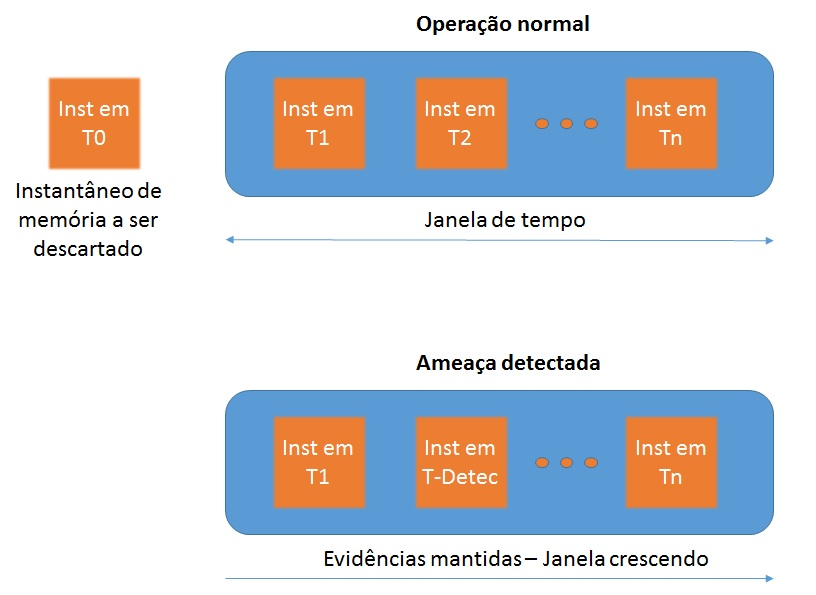
\includegraphics[scale=0.4]{janela.jpg}
\centering
\label{fig:janela}
\end{figure}

De modo a não violar a jurisdição de outros países ou a privacidade de outros usuários por causa do caráter multi-inquilino e multi-jurisdição das arquiteturas em nuvem pública, a solução proposta foi o de armazenar a evidência em um local físico fora da nuvem utilizando como transporte uma conexão segura. 
%
Outro ponto importante é garantir que a evidência não foi destruída, alterada ou acessada por qualquer pessoa. 
%
Assim a solução proposta por este trabalho usará de armazenamento físico fora da nuvem, o transporte será feito por TLS, no momento do armazenamento será calculado o hash da evidência e o acesso ao mesmo será controlado.

Tendo a implementação sido bem sucedida será possível analisar e identificar as formas de ataque enumeradas nos objetivos.\\

\subsection{Implementação}

A implementação da solução foi realizada em um notebook intel I5 de 2.30Mhz e 4Gb de RAM com sistema operacional de 64 bits. 
%
Nele, usando Oracle Virtual Box 5.0 foi criada uma máquina virtual com 2 Gb de memória RAM emulando apenas 1 processador.
%
Na máquina virtual foi instalada a versão 1.10 do Docker engine e 1.21 da API, criados 3 contêiners, cada um rodando um nginx 1.0 em diferentes portas. 
%
Escreveu-se uma aplicação em JAVA que descobre qual o PID associado a cada contêiner e salva o \textbf{/proc/pid/numa\_maps} em um arquivo.
%
A cópia e gravação do arquivo acontece da seguinte forma: a cada minuto a aplicação pausa o contêiner em questão, tira uma cópia do numa\_maps, salva em um arquivo .mem e concatenavcom o hash de identificação da imagem. 
%
Em seguida verifica qual o arquivo .mem mais antigo em disco, se for mais velho que o tempo 't', o arquivo é descartado.

\subsection{Limitações}

A solução esta focada em coletar informações de memória do user space, ela não enxerga o kernel space. 
%
Técnicas de investigação de malware que se baseam em informações do kernel space como por exemplo, a comparação de informações do Process Environment Block (PEB), que ficam no user space, com informações do Virtual Address Descriptor (VAD), que fica no Kernel space não são possíveis. 
%
Outro exemplo é a análise de ameaças que realizam manipulação direta dos objetos do kernel ( \textit{D.K.O.M. - Direct Kernel Object Manipulation} ) também não se beneficiam de associação com o contêiner.

A solução completa com todos os elementos descritos anteriormente pode ser visto na figura 4

\begin{figure}[h]
\caption{Solução completa}
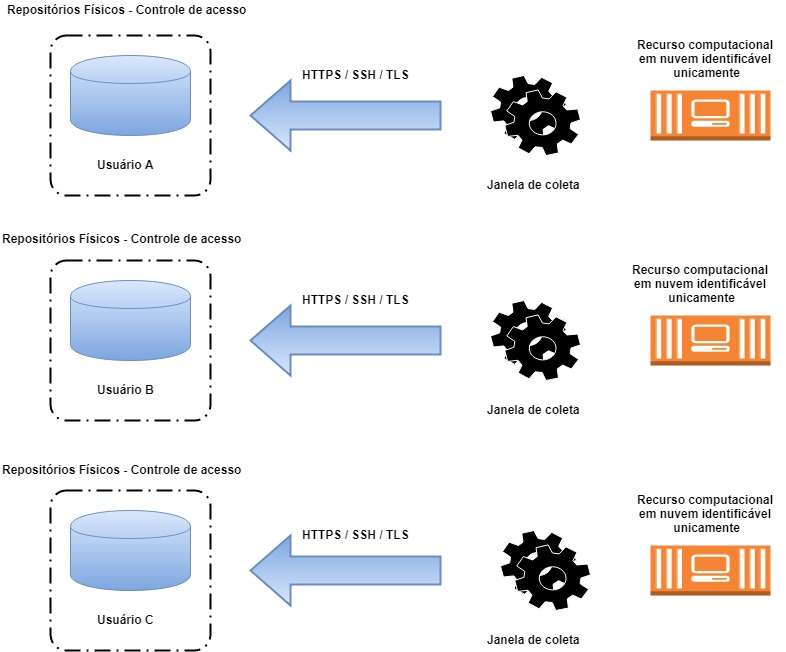
\includegraphics[scale=0.25]{solucao.jpg}
\label{fig:Solucao}
\end{figure}

% An example of a floating figure using the graphicx package.
% Note that \label must occur AFTER (or within) \caption.
% For figures, \caption should occur after the \includegraphics.
% Note that IEEEtran v1.7 and later has special internal code that
% is designed to preserve the operation of \label within \caption
% even when the captionsoff option is in effect. However, because
% of issues like this, it may be the safest practice to put all your
% \label just after \caption rather than within \caption{}.
%
% Reminder: the "draftcls" or "draftclsnofoot", not "draft", class
% option should be used if it is desired that the figures are to be
% displayed while in draft mode.
%
%\begin{figure}[!t]
%\centering
%\includegraphics[width=2.5in]{myfigure}
% where an .eps filename suffix will be assumed under latex, 
% and a .pdf suffix will be assumed for pdflatex; or what has been declared
% via \DeclareGraphicsExtensions.
%\caption{Simulation Results.}
%\label{fig_sim}
%\end{figure}

% Note that IEEE typically puts floats only at the top, even when this
% results in a large percentage of a column being occupied by floats.


% An example of a double column floating figure using two subfigures.
% (The subfig.sty package must be loaded for this to work.)
% The subfigure \label commands are set within each subfloat command,
% and the \label for the overall figure must come after \caption.
% \hfil is used as a separator to get equal spacing.
% Watch out that the combined width of all the subfigures on a 
% line do not exceed the text width or a line break will occur.
%
%\begin{figure*}[!t]
%\centering
%\subfloat[Case I]{\includegraphics[width=2.5in]{box}%
%\label{fig_first_case}}
%\hfil
%\subfloat[Case II]{\includegraphics[width=2.5in]{box}%
%\label{fig_second_case}}
%\caption{Simulation results.}
%\label{fig_sim}
%\end{figure*}
%
% Note that often IEEE papers with subfigures do not employ subfigure
% captions (using the optional argument to \subfloat[]), but instead will
% reference/describe all of them (a), (b), etc., within the main caption.


% An example of a floating table. Note that, for IEEE style tables, the 
% \caption command should come BEFORE the table. Table text will default to
% \footnotesize as IEEE normally uses this smaller font for tables.
% The \label must come after \caption as always.
%
%\begin{table}[!t]
%% increase table row spacing, adjust to taste
%\renewcommand{\arraystretch}{1.3}
% if using array.sty, it might be a good idea to tweak the value of
% \extrarowheight as needed to properly center the text within the cells
%\caption{An Example of a Table}
%\label{table_example}
%\centering
%% Some packages, such as MDW tools, offer better commands for making tables
%% than the plain LaTeX2e tabular which is used here.
%\begin{tabular}{|c||c|}
%\hline
%One & Two\\
%\hline
%Three & Four\\
%\hline
%\end{tabular}
%\end{table}


% Note that IEEE does not put floats in the very first column - or typically
% anywhere on the first page for that matter. Also, in-text middle ("here")
% positioning is not used. Most IEEE journals/conferences use top floats
% exclusively. Note that, LaTeX2e, unlike IEEE journals/conferences, places
% footnotes above bottom floats. This can be corrected via the \fnbelowfloat
% command of the stfloats package.

\section{Conclusoes Finais}
\label{sec:conclusion}

Até o momento a presente proposta teve sucesso em relacionar o instantâneo de memória a sua origem através do hash de identificação da imagem, usou-se a versão 1.10 do Docker para tal fim. 
%
A versão é importante pois até a 1.9.x, o identificador da imagem era apenas um randômico. Na versão 1.10 ele passou a ser um hash calculado a partir da imagem.

Apesar do sucesso em salvar a memória relacionadas ao contêiner e sua associação com a origem, não foi possível até o momento relizar uma análise das ameaças. 
%
As ferramentas de leitura de memória disponíveis no mercado requerem que todo o conteúdo da memória da máquina esteja disponível para realização da análise. 
%
Como é coletada apenas a memória relacionada aos processos, o ferramental não funciona. 
%
É necessário o desenvolvimento de uma ferramenta que trabalhe sem a memória completa da máquina, ou no caso da ferramenta \textit{Volatility} é necessário a criação de um profile para a memória do processo

% trigger a \newpage just before the given reference
% number - used to balance the columns on the last page
% adjust value as needed - may need to be readjusted if
% the document is modified later
%\IEEEtriggeratref{8}
% The "triggered" command can be changed if desired:
%\IEEEtriggercmd{\enlargethispage{-5in}}

% references section

% can use a bibliography generated by BibTeX as a .bbl file
% BibTeX documentation can be easily obtained at:
% http://www.ctan.org/tex-archive/biblio/bibtex/contrib/doc/
% The IEEEtran BibTeX style support page is at:
% http://www.michaelshell.org/tex/ieeetran/bibtex/
\bibliographystyle{IEEEtran}
% argument is your BibTeX string definitions and bibliography database(s)
\bibliography{IEEEabrv,artigo-ieee.bib}

% <OR> manually copy in the resultant .bbl file
% set second argument of \begin to the number of references
% (used to reserve space for the reference number labels box)

\end{document}


